\newcommand{\rTc}{\varsigma}
\newcommand{\fractt}[2]{\frac{\text{#1}}{\text{#2}}}
\newcommand{\rTt}{\vartheta}
\newcommand{\Ce}{\mathbf{C}_e}
\newcommand{\veltriangle}{%
  \begingroup\normalfont
  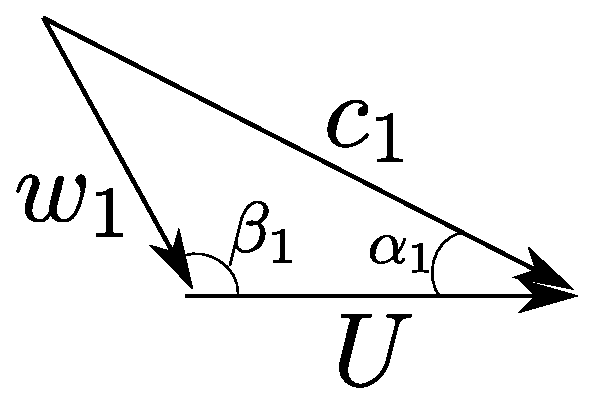
\includegraphics[height=2\fontcharht\font`\B]{triangulo.eps}%
  \endgroup
}
\begin{formuleo}[Fundamentalismos]
Euler:  $-\frac{\dot{W}}{\dot{m}}=\tau\cdot \Omega=-e=U_{2} \ctan{2}-U_{1} \ctan{1} =\left(h_{02}-h_{01}\right)=\left(\frac{c_{2}^{2}-c_{1}^{2}}{2}\right)+\left(\frac{U_{2}^{2}-U_{1}^{2}}{2}\right)+\left(\frac{w_{1}^{2}-w_{2}^{2}}{2}\right)$    \\
Primera Ley: $ \dot{U}=\dot{Q}-\dot{W} - \dot{m}\left[\left(h_{2}-h_{1}\right)+\frac{1}{2}\left(c_{2}^{2}-c_{1}^{2}\right)+g\left(z_{2}-z_{1}\right)\right]$
Rend. de la instalación: $\frac{\text{Potencia efectiva}}{\text{Potencia entregada a la instalación}}$    \\
\textbf{Ley de Coseno:} $c^2 = a^2+b^2 - 2ab\cos{\theta_{\widehat{ab}}}$
\end{formuleo}


\formuleoseparator


\begin{formuleo}[T. Hidráulicas]
Pelton: aprox Dixon $w_2\approx U\rightarrow$ $c_2 \approx 2 U \sin \frac{\beta_2}{2}$ donde $\beta_{2}=180^\circ-\vartheta_{2}$ \ $\eta_{\mathrm{h}}^{\mathrm{pelton}}=\frac{U\left(c_{1}-c_{\theta 2}\right)}{g H}$    \\
Kaplan: $\cax{1}=\cax{2} = \frac{Q}{\pi(r_{\mathrm{ext}}^2-r_{\mathrm{int}}^2)}$ \separar $\eta_{\mathrm{h}}^{\mathrm{kaplan}} = \frac{\dW/\dm}{gH}$    \\
$\text{Eficiencia Hidráulica} = \fractt{Potencia entregada al rotor}{Potencia que se puede entregar a la instalación (potencial)}$
\end{formuleo}


\formuleoseparator


\begin{formuleo}[T. de Vapor]
Trabajo: $\mathrm{d} e=\frac{1}{\rho} \mathrm{d} p+\mathrm{d} \frac{1}{2} c^{2}+\mathrm{d} q$\separar
Tobera: $\eta_{\mathrm{iso}}^{\mathrm{tobera}}=\frac{c_{1}^{2} / 2}{c_{1 s}^{2} / 2}$; $K_{f}=\frac{c_{1}}{c_{1 s}}$ \separar 
Rotor: $dp=0:\ \eta_{\mathrm{iso}}^{\mathrm{rotor}}=\frac{\dot{W} / \dot{m}}{c_{1}^{2} / 2}$ con $K_{m}=\frac{w_{2}}{w_{1}}$ \separar Eficiencia interna de etapa: $\eta_{i}=\eta_{\mathrm{iso}}^{\mathrm{tobera}} \cdot \eta_{\mathrm{liso}}^{\mathrm{rotor}} \cdot \ldots=\frac{\dW / \dot{m}}{\Delta h_{s}}$ Eficiencia maxima: $\frac{U}{c_{1}}=\frac{\cos \alpha_{1}}{2m \cdot(1-\degreeofreaction)} $ \\ 
\textbf{Escalonamiento de reacción}. Fijo: $c_{2s}=\sqrt{2 \Delta h_{s}(1-\degreeofreaction )+c_{1}^{2}}$  Movil: $w_{2s}=\sqrt{2 \Delta h_{s}\degreeofreaction +
w_{1}^{2}}$ donde $K_m = \frac{w_2}{w_{2s}}$\\ Perdidas tobera: $Y_{\mathrm{tob.}}=\dot{m}(c^2_{1s}/2-c^2_1/2)$  Perdidas movil: $Y_{\mathrm{m}} = \dot{m}(w_1^2/2 - w_2^2/2)$
Perdidas roz. entre fijo/movil: $k_{\mathrm{axial}}=0,009$ ,$k_{\mathrm{radial}}=0,027$ : $Y_{\mathrm{roz.}}=k \rho n_{\mathrm{Hz}}^{3} D_m^{5}$ [W]\separar Perdidas ventil. $\varepsilon$ es grado adm. $l$ es largo alabes en \emph{cm}, $D_m$ es diametro medio y $k$ depende del nro. de ruedas $k_1=3,8$; $k_2=4,5$; $k_3=6 \going $ $Y_{\mathrm{vent.}}=(1-\varepsilon) k \rho n^{3} D_m^{4} l$ [W].  donde $\varepsilon = \fractt{Long arco inyeccion}{circunferencia media (U/omega)}$ donde $\ell_a = \frac{\dm}{\rho h c_0}$ para una ÚNICA tobera cuadrada $A=\ell_a \cdot h$  \\
Etapa acción: $c_0\approx 0$ para tobera. Rend. Maximo de UNA etapa accion ($c_1$ salida tobera): $\eta_{\max} = \frac{\dW/\dm}{c_{1s}^2/2}= K_f^2 \cdot \frac{\cos^2(\alpha_1)}{2}\cdot (1+K_m \frac{\cos \beta_1}{\cos \beta_2})$
\end{formuleo}


\formuleoseparator


\begin{formuleo}[T.Gas]
Valores: ${\cp}_{comb} \approx 1,15$ [kJ/kg]; $\ctegas_{comb.} \approx 1,33$; $\eta_{\mathrm{comb}} = \frac{\operatorname{FAC}_t}{\operatorname{FAC}_c}$

Relacion de compresion (Segun Hilal): $\relcomp = \frac{p_2}{p_1}$  Potencia eff donde $w=\Delta h$    \\
$\dot{W}_{e}=\left(\dot{m}_{\mathrm{air}}+\dot{m}_{\mathrm{comb.}}\right) \cdot |w_{\mathrm{turb.}}|-\dot{m}_{\mathrm{air}} \cdot |w_{\mathrm{comp.}}|$ donde $w_t = h_{\mathrm{in}}-h_{\mathrm{out}}={\cp}_{\mathrm{cte}} (T_{\mathrm{in}}-T_{\mathrm{out}}) $ \\
Eficiencias Internas: $\etaint^{\mathrm{turb.}} = \fractt{Potencia ciclo indicado}{Potencia ciclo ideal} = \frac{\Delta h}{\Delta h_s}$     Efic. mecánicas(al reves para bombas): $\etamec^{\mathrm{turb.}} = \fractt{Potencia entregada}{Potencia indicada} = \frac{w_t}{w^{\mathrm{ind}}_{t}} $    \\
Optimo $\rTc$: $\relcomp^* =\left(\frac{T_{3}}{T_{1}} \eta_{c} \eta_{t} \frac{c_{34}}{c_{12}}\right)^{\left(\frac{\ctegas}{2(\ctegas-1)}\right)}$
Regeneración: $\sigma=\frac{T_A-T_2}{T_4 - T_2}$,$\rTc = \frac{T_2}{T_1}$,$\rTt=\frac{T_3}{T_1}$,$\eta_{\mathrm{regen}} = \frac{\rTc  -1}{\rTc} \frac{\rTt-\rTc}{\rTt -\rTc - \sigma \frac{\rTt - \rTc^2}{\rTc}} $ 
\separar Poder Calorico del combustible (PCI) [J/kg] Consumo especifico $\Ce = \frac{\dot{m}_{\mathrm{comb.}}}{P_e}\going$ $\eta_{\mathrm{instalacion}} = \frac{\dW_e}{\dot{m}_{\mathrm{comb.}} \cdot \mathrm{PCI}}=\frac{1}{\Ce \cdot\mathrm{PCI}}$   \\

\end{formuleo}


\formuleoseparator


\begin{formuleo}[Ciclo combinado]
Rankine: $\eta=\frac{\dot{W}_{\mathrm{t}} / \dot{m}-\dot{W}_{\mathrm{b}} / \dot{m}}{\dot{Q}_{\mathrm{in}} / \dot{m}}=\frac{\left|\Delta h_{\mathrm{turb} .}\right|-\Delta h_{\mathrm{bomba}}}{\Delta h_{\mathrm{cald}}}=1-\frac{\left|\Delta h_{\mathrm{cond} .}\right|}{\Delta h_{\mathrm{cald}}}$\separar $\mathrm{BWR}=\frac{\dot{W}_{\mathrm{b}} / \dot{m}}{\dot{W}_{\mathrm{t}} / \dot{m}}=\frac{\Delta h_{\mathrm{bomba}}}{ | \Delta h_{\mathrm{turb}} |}$ \separar Turb/bomba ($b$ al revés): $\eta_{\mathrm{t}}=\frac{\Delta h_{\text { turb }}}{\left(\Delta h_{\text { turb. }}\right)_{s}}$
\veltriangle
\end{formuleo}
\formuleoseparator

% Cosas que faltaron: Brayton formas de aumentar potencia/rendimiento y como influia cada una la potencia/rendimiento

%
